\documentclass{standalone}
\usepackage{tikz}
\usetikzlibrary{patterns, positioning}


\begin{document}
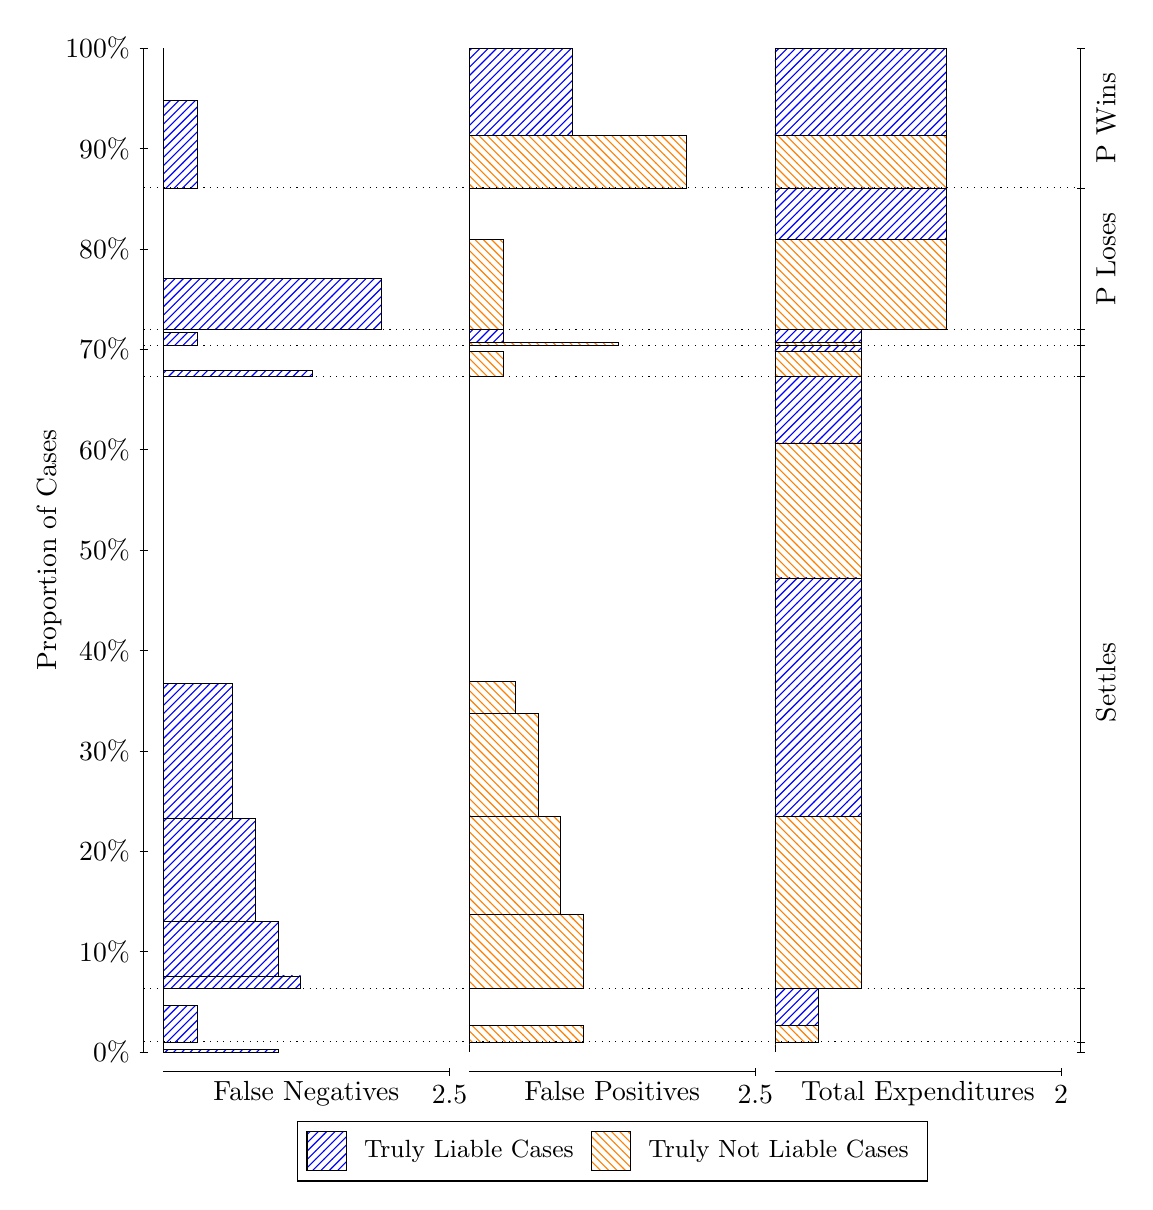
\begin{tikzpicture}
\draw[black, very thin] (1.5,1.75) -- (1.5,14.5);
\node[rotate=90, text=black, anchor=center] at (0.3, 8.125) {Proportion of Cases};
\draw[black, very thin] (1.45,1.75) -- (1.55,1.75);
\node[text=black, anchor=east] at (1.45, 1.75) {0\%};
\draw[black, very thin] (1.45,3.025) -- (1.55,3.025);
\node[text=black, anchor=east] at (1.45, 3.025) {10\%};
\draw[black, very thin] (1.45,4.3) -- (1.55,4.3);
\node[text=black, anchor=east] at (1.45, 4.3) {20\%};
\draw[black, very thin] (1.45,5.575) -- (1.55,5.575);
\node[text=black, anchor=east] at (1.45, 5.575) {30\%};
\draw[black, very thin] (1.45,6.85) -- (1.55,6.85);
\node[text=black, anchor=east] at (1.45, 6.85) {40\%};
\draw[black, very thin] (1.45,8.125) -- (1.55,8.125);
\node[text=black, anchor=east] at (1.45, 8.125) {50\%};
\draw[black, very thin] (1.45,9.4) -- (1.55,9.4);
\node[text=black, anchor=east] at (1.45, 9.4) {60\%};
\draw[black, very thin] (1.45,10.675) -- (1.55,10.675);
\node[text=black, anchor=east] at (1.45, 10.675) {70\%};
\draw[black, very thin] (1.45,11.95) -- (1.55,11.95);
\node[text=black, anchor=east] at (1.45, 11.95) {80\%};
\draw[black, very thin] (1.45,13.225) -- (1.55,13.225);
\node[text=black, anchor=east] at (1.45, 13.225) {90\%};
\draw[black, very thin] (1.45,14.5) -- (1.55,14.5);
\node[text=black, anchor=east] at (1.45, 14.5) {100\%};

\draw[black, very thin] (13.4,1.75) -- (13.4,14.5);
\draw[black, very thin] (13.35,1.75) -- (13.45,1.75);
\node[anchor=west] at (13.35, 1.75) {};
\draw[black, very thin] (13.35,1.8791) -- (13.45,1.8791);
\node[anchor=west] at (13.35, 1.8791) {};
\draw[black, very thin] (13.35,2.5595) -- (13.45,2.5595);
\node[anchor=west] at (13.35, 2.5595) {};
\draw[black, very thin] (13.35,10.331) -- (13.45,10.331);
\node[anchor=west] at (13.35, 10.331) {};
\draw[black, very thin] (13.35,10.726) -- (13.45,10.726);
\node[anchor=west] at (13.35, 10.726) {};
\draw[black, very thin] (13.35,10.923) -- (13.45,10.923);
\node[anchor=west] at (13.35, 10.923) {};
\draw[black, very thin] (13.35,12.724) -- (13.45,12.724);
\node[anchor=west] at (13.35, 12.724) {};
\draw[black, very thin] (13.35,14.5) -- (13.45,14.5);
\node[anchor=west] at (13.35, 14.5) {};

\draw[black, very thin, pattern color=blue, pattern=north east lines] (1.75,1.75) rectangle (3.2033,1.7854);
\draw[black, very thin, pattern color=orange, pattern=north west lines] (1.75,1.7854) rectangle (1.75,1.8791);
\draw[black, very thin, pattern color=blue, pattern=north east lines] (1.75,1.8791) rectangle (2.186,2.3466);
\draw[black, very thin, pattern color=orange, pattern=north west lines] (1.75,2.3466) rectangle (1.75,2.5595);
\draw[black, very thin, pattern color=blue, pattern=north east lines] (1.75,2.5595) rectangle (3.494,2.7151);
\draw[black, very thin, pattern color=blue, pattern=north east lines] (1.75,2.7151) rectangle (3.2033,3.4054);
\draw[black, very thin, pattern color=blue, pattern=north east lines] (1.75,3.4054) rectangle (2.9127,4.716);
\draw[black, very thin, pattern color=blue, pattern=north east lines] (1.75,4.716) rectangle (2.622,6.4308);
\draw[black, very thin, pattern color=orange, pattern=north west lines] (1.75,6.4308) rectangle (1.75,10.331);
\draw[black, very thin, pattern color=blue, pattern=north east lines] (1.75,10.331) rectangle (3.6393,10.408);
\draw[black, very thin, pattern color=orange, pattern=north west lines] (1.75,10.408) rectangle (1.75,10.726);
\draw[black, very thin, pattern color=blue, pattern=north east lines] (1.75,10.726) rectangle (2.186,10.884);
\draw[black, very thin, pattern color=orange, pattern=north west lines] (1.75,10.884) rectangle (1.75,10.923);
\draw[black, very thin, pattern color=blue, pattern=north east lines] (1.75,10.923) rectangle (4.5113,11.576);
\draw[black, very thin, pattern color=orange, pattern=north west lines] (1.75,11.576) rectangle (1.75,12.724);
\draw[black, very thin, pattern color=blue, pattern=north east lines] (1.75,12.724) rectangle (2.186,13.836);
\draw[black, very thin, pattern color=orange, pattern=north west lines] (1.75,13.836) rectangle (1.75,14.5);
\draw[black, very thin, pattern color=orange, pattern=north west lines] (5.6333,1.75) rectangle (5.6333,1.8437);
\draw[black, very thin, pattern color=blue, pattern=north east lines] (5.6333,1.8437) rectangle (5.6333,1.8791);
\draw[black, very thin, pattern color=orange, pattern=north west lines] (5.6333,1.8791) rectangle (7.0867,2.0921);
\draw[black, very thin, pattern color=blue, pattern=north east lines] (5.6333,2.0921) rectangle (5.6333,2.5595);
\draw[black, very thin, pattern color=orange, pattern=north west lines] (5.6333,2.5595) rectangle (7.0867,3.4954);
\draw[black, very thin, pattern color=orange, pattern=north west lines] (5.6333,3.4954) rectangle (6.796,4.7466);
\draw[black, very thin, pattern color=orange, pattern=north west lines] (5.6333,4.7466) rectangle (6.5053,6.0543);
\draw[black, very thin, pattern color=orange, pattern=north west lines] (5.6333,6.0543) rectangle (6.2147,6.4596);
\draw[black, very thin, pattern color=blue, pattern=north east lines] (5.6333,6.4596) rectangle (5.6333,10.331);
\draw[black, very thin, pattern color=orange, pattern=north west lines] (5.6333,10.331) rectangle (6.0693,10.648);
\draw[black, very thin, pattern color=blue, pattern=north east lines] (5.6333,10.648) rectangle (5.6333,10.726);
\draw[black, very thin, pattern color=orange, pattern=north west lines] (5.6333,10.726) rectangle (7.5227,10.764);
\draw[black, very thin, pattern color=blue, pattern=north east lines] (5.6333,10.764) rectangle (6.0693,10.923);
\draw[black, very thin, pattern color=orange, pattern=north west lines] (5.6333,10.923) rectangle (6.0693,12.071);
\draw[black, very thin, pattern color=blue, pattern=north east lines] (5.6333,12.071) rectangle (5.6333,12.724);
\draw[black, very thin, pattern color=orange, pattern=north west lines] (5.6333,12.724) rectangle (8.3947,13.388);
\draw[black, very thin, pattern color=blue, pattern=north east lines] (5.6333,13.388) rectangle (6.9413,14.5);
\draw[black, very thin, pattern color=orange, pattern=north west lines] (9.5167,1.75) rectangle (9.5167,1.8437);
\draw[black, very thin, pattern color=blue, pattern=north east lines] (9.5167,1.8437) rectangle (9.5167,1.8791);
\draw[black, very thin, pattern color=orange, pattern=north west lines] (9.5167,1.8791) rectangle (10.062,2.0921);
\draw[black, very thin, pattern color=blue, pattern=north east lines] (9.5167,2.0921) rectangle (10.062,2.5595);
\draw[black, very thin, pattern color=orange, pattern=north west lines] (9.5167,2.5595) rectangle (10.607,4.7466);
\draw[black, very thin, pattern color=blue, pattern=north east lines] (9.5167,4.7466) rectangle (10.607,7.772);
\draw[black, very thin, pattern color=orange, pattern=north west lines] (9.5167,7.772) rectangle (10.607,9.485);
\draw[black, very thin, pattern color=blue, pattern=north east lines] (9.5167,9.485) rectangle (10.607,10.331);
\draw[black, very thin, pattern color=orange, pattern=north west lines] (9.5167,10.331) rectangle (10.607,10.648);
\draw[black, very thin, pattern color=blue, pattern=north east lines] (9.5167,10.648) rectangle (10.607,10.726);
\draw[black, very thin, pattern color=orange, pattern=north west lines] (9.5167,10.726) rectangle (10.607,10.764);
\draw[black, very thin, pattern color=blue, pattern=north east lines] (9.5167,10.764) rectangle (10.607,10.923);
\draw[black, very thin, pattern color=orange, pattern=north west lines] (9.5167,10.923) rectangle (11.697,12.071);
\draw[black, very thin, pattern color=blue, pattern=north east lines] (9.5167,12.071) rectangle (11.697,12.724);
\draw[black, very thin, pattern color=orange, pattern=north west lines] (9.5167,12.724) rectangle (11.697,13.388);
\draw[black, very thin, pattern color=blue, pattern=north east lines] (9.5167,13.388) rectangle (11.697,14.5);
\draw[black, dotted] (1.5,1.8791) -- (13.4,1.8791);
\draw[black, dotted] (1.5,2.5595) -- (13.4,2.5595);
\draw[black, dotted] (1.5,10.331) -- (13.4,10.331);
\draw[black, dotted] (1.5,10.726) -- (13.4,10.726);
\draw[black, dotted] (1.5,10.923) -- (13.4,10.923);
\draw[black, dotted] (1.5,12.724) -- (13.4,12.724);
\draw[black, very thin] (1.75,1.5) -- (5.3833,1.5);
\node[text=black, anchor=north] at (3.5667, 1.5) {False Negatives};
\draw[black, very thin] (5.3833,1.45) -- (5.3833,1.55);
\node[text=black, anchor=north] at (5.3833, 1.45) {2.5};

\draw[black, very thin] (5.6333,1.5) -- (9.2667,1.5);
\node[text=black, anchor=north] at (7.45, 1.5) {False Positives};
\draw[black, very thin] (9.2667,1.45) -- (9.2667,1.55);
\node[text=black, anchor=north] at (9.2667, 1.45) {2.5};

\draw[black, very thin] (9.5167,1.5) -- (13.15,1.5);
\node[text=black, anchor=north] at (11.333, 1.5) {Total Expenditures};
\draw[black, very thin] (13.15,1.45) -- (13.15,1.55);
\node[text=black, anchor=north] at (13.15, 1.45) {2};



\node[text=black, centered, rotate=90] at (13.72, 6.4452) {Settles};


\node[text=black, centered, rotate=90] at (13.72, 11.823) {P Loses};
\node[text=black, centered, rotate=90] at (13.72, 13.612) {P Wins};

\draw (7.449999999999999,1.5) node[draw=none] (baseCoordinate) {};
\begin{scope}[align=center]
        \matrix[scale=0.5, draw=black, below=0.5cm of baseCoordinate, nodes={draw}, column sep=0.1cm]{
            \node[rectangle, draw, minimum width=0.5cm, minimum height=0.5cm, pattern color=blue, pattern=north east lines] {}; &
            \node[draw=none, font=\small, text=black] (B) {Truly Liable Cases}; &
            \node[rectangle, draw, minimum width=0.5cm, minimum height=0.5cm, pattern color=orange, pattern=north west lines] {}; &
            \node[draw=none, font=\small, text=black] (B) {Truly Not Liable Cases}; \\
            };
\end{scope}

\end{tikzpicture}
\end{document}